% This example is meant to be compiled with lualatex or xelatex
% The theme itself also supports pdflatex
\PassOptionsToPackage{unicode}{hyperref}
\documentclass[aspectratio=1610, 12pt, xcolor=dvipsnames]{beamer}

% Warning, if another latex run is needed
% \usepackage[aux]{rerunfilecheck}

% just list chapters and sections in the toc, not subsections or smaller
\setcounter{tocdepth}{1}

%------------------------------------------------------------------------------
%------------------------------ Fonts, Unicode, Language ----------------------
%------------------------------------------------------------------------------
\usepackage{fontspec}
\defaultfontfeatures{Ligatures=TeX}  % -- becomes en-dash etc.

% german language
\usepackage{polyglossia}
\setdefaultlanguage{german}

% for english abstract and english titles in the toc
\setotherlanguages{english}

% intelligent quotation marks, language and nesting sensitive
\usepackage[autostyle]{csquotes}

% microtypographical features, makes the text look nicer on the small scale
\usepackage{microtype}

% colors and stuff
\usepackage{xcolor}
\usepackage[most]{tcolorbox}
\tcbset{on line, hbox,
        boxsep=4pt, left=0pt,right=0pt,top=0pt,bottom=0pt,
        colframe=white,colback=SpringGreen,  
        highlight math style={enhanced}
        }
\newtcolorbox{mybox}[3][]
{
  colframe = #2!25,
  colback = #2!20,
  coltitle = #2!20!black,
  title = {#3},
  #1
}
%\colorlet{Green!40}
%------------------------------------------------------------------------------
%------------------------ Math Packages and settings --------------------------
%------------------------------------------------------------------------------

\usepackage{amsmath}
\usepackage{amssymb}
\usepackage{mathtools}
\usepackage{bbold}

% Enable Unicode-Math and follow the ISO-Standards for typesetting math
\usepackage[
  math-style=ISO,
  bold-style=ISO,
  sans-style=italic,
  nabla=upright,
  partial=upright,
]{unicode-math}
\setmathfont{Latin Modern Math}

% nice, small fracs for the text with \sfrac{}{}
\usepackage{xfrac}


%------------------------------------------------------------------------------
%---------------------------- Numbers and Units -------------------------------
%------------------------------------------------------------------------------

\usepackage[
  locale=DE,
  separate-uncertainty=true,
  per-mode=symbol-or-fraction,
]{siunitx}
\sisetup{math-micro=\text{µ},text-micro=µ}
% \sisetup{tophrase={{ to }}}
%------------------------------------------------------------------------------
%-------------------------------- tables  -------------------------------------
%------------------------------------------------------------------------------

\usepackage{booktabs}       % \toprule, \midrule, \bottomrule, etc

%------------------------------------------------------------------------------
%-------------------------------- graphics -------------------------------------
%------------------------------------------------------------------------------

\usepackage{graphicx}
%\usepackage{rotating}
\usepackage{grffile}
\usepackage{tikz}
\usepackage{circuitikz}
\usepackage{tikz-feynman}
\usepackage{subcaption}

% allow figures to be placed in the running text by default:
\usepackage{scrhack}
\usepackage{float}
\floatplacement{figure}{htbp}
\floatplacement{table}{htbp}

% keep figures and tables in the section
\usepackage[section, below]{placeins}

% smileys
\usepackage{MnSymbol,wasysym}

%------------------------------------------------------------------------------
%---------------------- customize list environments ---------------------------
%------------------------------------------------------------------------------

\usepackage{enumitem}
\usepackage{listings}
\usepackage{hepunits}

\usepackage{pdfpages}
%------------------------------------------------------------------------------
%------------------------------ Bibliographie ---------------------------------
%------------------------------------------------------------------------------

\usepackage[
  backend=biber,   % use modern biber backend
  autolang=hyphen, % load hyphenation rules for if language of bibentry is not
                   % german, has to be loaded with \setotherlanguages
                   % in the references.bib use langid={en} for english sources
]{biblatex}
\addbibresource{references.bib}  % the bib file to use
\DefineBibliographyStrings{german}{andothers = {{et\,al\adddot}}}  % replace u.a. with et al.


% Load packages you need here
% \usepackage{polyglossia}
% \setmainlanguage{german}

\usepackage{csquotes}


% \usepackage{amsmath}
% \usepackage{amssymb}
% \usepackage{mathtools}

\usepackage{hyperref}
\usepackage{bookmark}

% load the theme after all packages

\usetheme[
  showtotalframes, % show total number of frames in the footline
]{tudo}

% Put settings here, like
\unimathsetup{
  math-style=ISO,
  bold-style=ISO,
  nabla=upright,
  partial=upright,
  mathrm=sym,
}

% \setbeamertemplate{itemize item}{\scriptsize$\blacktriangleright$}
% \setbeamertemplate{itemize subitem}{\scriptsize$\blacktriangleright$}

%Titel:
\title{Global alignment of the LHCb SciFi Tracker and Vertex Locator}
%Autor
\author[N.Breer]{\textbf{Nils Breer}, Biljana Mitreska, Sophie Hollitt, Johannes Albrecht}
%Lehrstuhl/Fakultät
\institute{DPG Conference, Karlsruhe}
%Titelgrafik muss ich einfueren!!!
%\titlegraphic{\includegraphics[width=0.3\textwidth]{content/Bilder/interferenz.jpg}}
\date{04.03.2024}

\begin{document}
\maketitle

\begin{frame}\frametitle{What is Alignment and why do we need it?}
  \begin{columns}
    \begin{column}[c]{0.48\textwidth}
      \input{detector.tex}
    \end{column}
    \begin{column}[c]{0.48\textwidth}
      \begin{itemize}
        \item $\bullet$\, Top: ideal detector, bottom: physical detector
        \item $\bullet$\, Surveys are used to find the rotation and position of each detector component
        \item $\bullet$\, \to Starting positions for software alignment
        \item $\bullet$\, Building tracks accurately requires positions in reconstruction to be as similar as possible to real positions
      \end{itemize}
    \end{column}
  \end{columns}
\end{frame}

\begin{frame}\frametitle{Importance of alignments}
  \begin{itemize}
    \item $\bullet$\, Alignment is part of the LHCb trigger system
    \item $\bullet$\, Physics performance tied to alignment performance
    \item $\bullet$\, with optimal alignment:
    \begin{itemize}
      \item $\bullet$\, \to\, remove systematic biases for asymmetry measurements
      \item $\bullet$\, Best possible mass resolution
    \end{itemize}
  \end{itemize}
  \begin{figure}
      \includegraphics[width=0.9\textwidth]{logos/dataflow.png}%
    % \caption{Hits on tracks in x-direction with run 256145 data on 20000 ents using 9 minimum hits against 11 minimum hits.}
  \end{figure}
\end{frame}

\begin{frame}\frametitle{Alignment: track fits with the Kalman Filter}
  \begin{columns}
    \begin{column}[c]{0.4\textwidth}
      \begin{figure}
        \centering
        \includegraphics[width=0.72\textwidth]{logos/kalman.png}
        % \caption{Alignment with Kalman Filter.}
      \end{figure}
    \end{column}
    \begin{column}[c]{0.55\textwidth}
      \begin{itemize}
        \item $\bullet$\, Starting positions: positions from laser scans of detector objects (survey)
        \item $\bullet$\, Alignment: $\chi^2$ minimization of track residuals
        \item $\bullet$\, Add measurements one-by-one to fit
        \item $\bullet$\, Prediction of next measurement \to minimize residuals \to redo until track complete
        \item $\bullet$\, Why Kalman Filter?
        \begin{itemize}
          \item $\bullet$\, easily models material interactions as well as multiple scattering
        \end{itemize}
      \end{itemize}
    \end{column}
  \end{columns}
\end{frame}

\begin{frame}\frametitle{LHCb upgraded with the SciFi}
  \begin{columns}
    \begin{column}[c]{0.48\textwidth}
      \begin{figure}
        \includegraphics[width=\textwidth]{logos/upgrade_lhcb.png}
        % \caption{Visualization of the SciFi tracking stations.}
      \end{figure}
    \end{column}
    \begin{column}{0.48\textwidth}
      \begin{itemize}
        \item $\bullet$\, 3 stations: T1, T2, T3
        \item $\bullet$\, 4 layers per station: X1, U, V, X2
      	\item $\bullet$\, Replaces former IT and OT to cope with the increased instantaneous luminosity
%	      \item $\bullet$\, crucial part of tracking system
      \end{itemize}
      \includegraphics[width=0.7\textwidth]{track.png}
    \end{column}
  \end{columns}
\end{frame}

\begin{frame}\frametitle{The Scintillating Fibre Tracker}
  \begin{columns}
    \begin{column}[c]{0.48\textwidth}
      \begin{figure}
        \includegraphics[width=0.9\textwidth]{logos/scifi.png}
        % \caption{Visualization of the SciFi tracking stations.}
      \end{figure}
    \end{column}
    \begin{column}{0.48\textwidth}
      \begin{itemize}
        \item $\bullet$\, Front two stations have 5 modules per side
        \item $\bullet$\, Back station has 6 modules on each side
        \item $\bullet$\, U, V layers have a $\mp 5 \deg$ stereo angle respectively
        \item $\bullet$\, \to\, Used for determining y-position of tracks by comparing hitposition at different angles
      \end{itemize}
    \end{column}
  \end{columns}
\end{frame}

% \begin{frame}\frametitle{Track hits comparison of V2 and simulation}
% \begin{mybox}{green}{}
%   \begin{itemize}
%     \item $\bullet$\, Simulation: hits on \textbf{reconstructed} tracks fill whole detector
%     \item $\bullet$\, A-side Track hits good!
%   \end{itemize}
% \end{mybox}
% \begin{mybox}{orange}{}
%   \begin{itemize}
%     \item \to\, Scan C-side quarters for possible issues in distinct layers
%   \end{itemize}
% \end{mybox}
%   \begin{columns}
%     \begin{column}[c]{0.48\textwidth}
%       \begin{figure}
%         \centering
%         \includegraphics[width=0.6\textwidth]{logos/nodeXY_MC.pdf}%
%       \end{figure}
%     \end{column}
%     \begin{column}[c]{0.48\textwidth}
%       \begin{figure}
%         \centering
%         \includegraphics[width=0.6\textwidth]{tuples_out/combining_2D_nodeXY_v2.pdf}%
%       \end{figure}
%     \end{column}
%   \end{columns}
% \end{frame}

\begin{frame}\frametitle{Global alignment and motivation}
  \begin{mybox}{green}{Global alignment}
    \begin{itemize}
      \item $\bullet$\, alignment of the velo and the scifi simultaneously
    \end{itemize}
    \begin{itemize}
      \setlength\itemsep{0em}
      \item $\bullet$\, Motivation for global alignment
      \begin{itemize}
        \item $\bullet$\, understanding the interplay between tracking systems
        \item $\bullet$\, rotations inside the VELO \to weak modes inside SciFi (VELO twisting)
      \end{itemize}
    \end{itemize}
  \end{mybox}
  \begin{mybox}{orange}{Configuration}
    \begin{itemize}
      \item First Longmodules then Halfmodules TxRxRz
      \item Full VELO RxRz + VELO halves TxTyTz
      \item VELO halves TxTyTz
      \item CFrames to be able to absorb for the average movement
      \item lagrage constraint in T2
      \item VELO backwards tracks
    \end{itemize}
  \end{mybox}
\end{frame}

\begin{frame}\frametitle{VELO global rotation}
  \begin{itemize}
    \item rotation Rz leading to shifts in x and y
    % \item half alignment somewhat sensitive and shows Rz ≈ 3 mrad
    \item half alignment sensitive to x shift 
    \item global movement in y
    \begin{itemize}
      \item can not be corrected for by half alignment
    \end{itemize}
  \end{itemize}
  \includegraphics[width=\textwidth]{plots/velo_rotation.png}
\end{frame}

\begin{frame}\frametitle{Comparison of SciFi only to global alignment}
  \begin{itemize}
    \setlength\itemsep{0em}
    \item $\bullet$\, zig-zag pattern still unknown origin
    \item \to correlated with Tz shifting showing similar trend
    \item $\bullet$\, small improvement in comparison to SciFi only
    \item \to layer movement has still issues from VELO rotation present in SciFi
  \end{itemize}
  \begin{columns}
    \begin{column}[c]{0.35\textwidth}
      \begin{figure}
        \centering
        \includegraphics[width=\textwidth]{plots/outfiles_vs_global/Layers_Tx_pattern.png}
      \end{figure}
    \end{column}
    \begin{column}[c]{0.5\textwidth}
      \begin{figure}
        \centering
        \includegraphics[width=\textwidth]{plots/outfiles_vs_global/all_runs_fix_glob_z_vs_local_Tx.pdf}
      \end{figure}
    \end{column}
  \end{columns}
\end{frame}

\begin{frame}\frametitle{Comparison of SciFi only to global alignment}
  \begin{columns}
    \begin{column}[c]{0.48\textwidth}
      \begin{figure}
        \centering
        \includegraphics[width=\textwidth]{plots/outfiles_vs_global/all_runs_fix_glob_z_vs_local_Rx.pdf}
      \end{figure}
    \end{column}
    \begin{column}[c]{0.48\textwidth}
      \begin{figure}
        \centering
        \includegraphics[width=\textwidth]{plots/outfiles_vs_global/all_runs_fix_glob_z_vs_local_Rz.pdf}
      \end{figure}
    \end{column}
  \end{columns}
\end{frame}

\begin{frame}\frametitle{Issues and possible solutions}
  \begin{itemize}
    \setlength\itemsep{0em}
    \item $\bullet$\, zig-zag pattern of stereo layers in Tx difficult to fix
    \item \to similar pattern in Tz \to cannot fix one without the other
    \item $\bullet$\, global VELO Rx might be overthrown by survey constrains acting on Rx \to Rx not being picked up in the alignment
    \item $\bullet$\, Testing different survey uncertanties to study the impact on global VELO rotation
    \item $\bullet$\, Testing different settings in the alignment on stereo layers in Tx
    \item make sure VELO Rx is being picked up in the alignment  \end{itemize}
\end{frame}


\begin{frame}\frametitle{Summary}
  \begin{itemize}
    \setlength\itemsep{0em}
    \item $\bullet$\, global alignment improving the position of the T-stations
    \item $\bullet$\, still unknown phenomena (zig-zag pattern, offset T2 position)
    \item $\bullet$\, survey constraints might counteract the global VELO Rx
    \item $\bullet$\, A lot more tests to do until data taking which look promising
    \item $\bullet$\, \textbf{Thank you for your attention!}
  \end{itemize}
  % \textbf{Thank you for your attention!}
\end{frame}

% \begin{frame}\frametitle{Backup: SciFi terminology}
%   Layers are divided into two halves commonly labeled as A-side and C-side
%   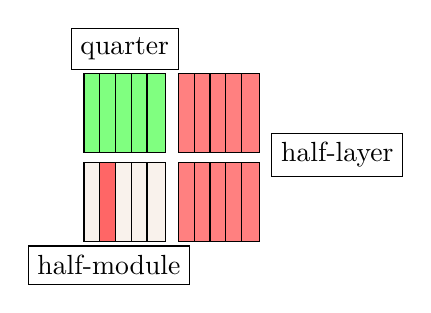
\begin{tikzpicture}
% first quarter
  \node[rectangle,
      draw = black,
      % text = ,
      fill = brown!10!white,
      minimum width = 0.2cm,
      minimum height = 1cm] (r) at (0,0) {};

  \node[rectangle,
      draw = black,
      % text = half-module,
      fill = red!60!white,
      minimum width = 0.2cm,
      minimum height = 1cm] (r) at (0.2,0) {};

  \node[rectangle,
      draw = black,
      % text = ,
      fill = brown!10!white,
      minimum width = 0.2cm,
      minimum height = 1cm] (r) at (0.4,0) {};

  \node[rectangle,
      draw = black,
      % text = ,
      fill = brown!10!white,
      minimum width = 0.2cm,
      minimum height = 1cm] (r) at (0.6,0) {};

  \node[rectangle,
      draw = black,
      % text = ,
      fill = brown!10!white,
      minimum width = 0.2cm,
      minimum height = 1cm] (r) at (0.8,0) {};

% second quarter
\node[rectangle,
    draw = black,
    % text = ,
    fill = red!50!white,
    minimum width = 0.2cm,
    minimum height = 1cm] (r) at (1.2,0) {};

\node[rectangle,
    draw = black,
    % text = ,
    fill = red!50!white,
    minimum width = 0.2cm,
    minimum height = 1cm] (r) at (1.4,0) {};

\node[rectangle,
    draw = black,
    % text = ,
    fill = red!50!white,
    minimum width = 0.2cm,
    minimum height = 1cm] (r) at (1.6,0) {};

\node[rectangle,
    draw = black,
    % text = ,
    fill = red!50!white,
    minimum width = 0.2cm,
    minimum height = 1cm] (r) at (1.8,0) {};

\node[rectangle,
    draw = black,
    % text = ,
    fill = red!50!white,
    minimum width = 0.2cm,
    minimum height = 1cm] (r) at (2,0) {};

% third quarter
\node[rectangle,
    draw = black,
    % text = ,
    fill = green!50!white,
    minimum width = 0.2cm,
    minimum height = 1cm] (r) at (0,1.13) {};

\node[rectangle,
    draw = black,
    % text = quarter,
    fill = green!50!white,
    minimum width = 0.2cm,
    minimum height = 1cm] (r) at (0.2,1.13) {};

\node[rectangle,
    draw = black,
    % text = ,
    fill = green!50!white,
    minimum width = 0.2cm,
    minimum height = 1cm] (r) at (0.4,1.13) {};

\node[rectangle,
    draw = black,
    % text = ,
    fill = green!50!white,
    minimum width = 0.2cm,
    minimum height = 1cm] (r) at (0.6,1.13) {};

\node[rectangle,
    draw = black,
    % text = ,
    fill = green!50!white,
    minimum width = 0.2cm,
    minimum height = 1cm] (r) at (0.8,1.13) {};

% fourth quarter
\node[rectangle,
    draw = black,
    % text = ,
    fill = red!50!white,
    minimum width = 0.2cm,
    minimum height = 1cm] (r) at (1.2,1.13) {};

\node[rectangle,
    draw = black,
    % text = ,
    fill = red!50!white,
    minimum width = 0.2cm,
    minimum height = 1cm] (r) at (1.4,1.13) {};

\node[rectangle,
    draw = black,
    % text = ,
    fill = red!50!white,
    minimum width = 0.2cm,
    minimum height = 1cm] (r) at (1.6,1.13) {};

\node[rectangle,
    draw = black,
    % text = ,
    fill = red!50!white,
    minimum width = 0.2cm,
    minimum height = 1cm] (r) at (1.8,1.13) {};

\node[rectangle,
    draw = black,
    % text = ,
    fill = red!50!white,
    minimum width = 0.2cm,
    minimum height = 1cm] (r) at (2,1.13) {};

\node[draw] at (0.4, 1.95) {quarter};
\node[draw] at (0.2, -0.8) {half-module};
\node[draw] at (3.1, 0.6) {half-layer};

\end{tikzpicture}

% \end{frame}

\begin{frame}\frametitle{The survey: what is it and the different types}
  \begin{columns}
    \begin{column}[c]{0.48\textwidth}
      $\bullet$\, Measure distance of some points on the detector with a laser
      \begin{figure}
        \centering
        \includegraphics[width=\textwidth]{logos/survey.png}
        % \caption{}
      \end{figure}
    \end{column}
    \begin{column}[c]{0.48\textwidth}
      \begin{itemize}
        \item $\bullet$\, Layer survey: find corners of layers
        \item $\bullet$\, Module survey: reflective stickers, calculate module plane
        \item $\bullet$\, Compare survey to simulation
      \end{itemize}
    \end{column}
  \end{columns}
\end{frame}


% not needed
% \begin{frame}\frametitle{Sources}
%   \begin{itemize}
%     \item $\bullet$\,SciFi Conference Talk: \url{https://twiki.cern.ch/twiki/pub/LHCb/SciFiConference/fee_2018.pdf}
%     \item $\bullet$\,LHCb SciFi: From performance requirements to an operational detector: \url{https://indico.cern.ch/event/1163878/}
%     \item $\bullet$\, BCAM \url{https://accelconf.web.cern.ch/ipac2018/papers/wepaf067.pdf}
%   \end{itemize}
% \end{frame}

\end{document}
